\documentclass[lettersize,journal]{IEEEtran}
\usepackage{amsmath,amsfonts}
\usepackage{algorithmic}
\usepackage{array}
\usepackage[caption=false,font=normalsize,labelfont=sf,textfont=sf]{subfig}
\usepackage{textcomp}
\usepackage{stfloats}
\usepackage{url}
\usepackage{verbatim}
\usepackage{graphicx}
\hyphenation{op-tical net-works semi-conduc-tor IEEE-Xplore}
\def\BibTeX{{\rm B\kern-.05em{\sc i\kern-.025em b}\kern-.08em
    T\kern-.1667em\lower.7ex\hbox{E}\kern-.125emX}}
\usepackage{balance}

\begin{document}
    \title{Real-Time Embedded Implementation of Winnerless Competition in a Discrete Nonlinear Neuromorphic System}
    
  \author{Luis Pabón-Orozco and Esther D. Gutiérrez.

  \thanks{Manuscript created June, 2026. (\textit{Corresponding author: Luis Pabón-Orozco}) }
  \thanks{Luis Pabón-Orozco and Esther D. Gutiérrez are with Escuela Superior Politécnica del Litoral, ESPOL, Facultad de Ciencias Naturales y Matematicas, Campus Gustavo Galindo km 30.5 Vía Perimetral, P.O. Box 09-01-5863, Guayaquil, Ecuador (e-mail: luispabo@espol.edu.ec).}
  }  
\maketitle
\begin{abstract}
Winnerless competition (WLC) is a dynamical regime characterized by sequential switching among metastable states without permanent dominance of a single unit, and has been associated with temporal encoding and pattern generation in nonlinear neural systems. Despite its theoretical relevance, embedded hardware realizations of WLC remain limited, particularly on low-cost and accessible platforms. This work presents a real-time embedded implementation of WLC using a three-neuron non-chaotic Rulkov network deployed on Arduino UNO microcontrollers. The proposed system distributes the network computation across independent embedded nodes, where each neuron updates its discrete-time dynamics locally and exchanges coupling signals with neighboring units. To preserve temporal consistency during distributed execution, a buffered state-update mechanism is introduced. Experimental results show that the hardware prototype reproduces the sequential switching and non-overlapping activation patterns predicted by numerical simulations for selected parameter configurations. The resulting dynamics are further associated with discrete symbolic motion codes, showing that WLC-like regimes can be exploited as an embedded low-cost encoding mechanism. These results provide a practical framework for the experimental study of discrete-time neuromorphic dynamics on accessible microcontroller-based platforms.
\end{abstract}
\begin{IEEEkeywords}
Winnerless competition, Rulkov map, neuromorphic computing, embedded systems, Arduino, nonlinear dynamics, discrete-time neural networks, symbolic encoding.
\end{IEEEkeywords}

\section{Introduction}
\IEEEPARstart{I}{n} nonlinear dynamical systems, the design of bio-inspired and neuromorphic computational architectures, where complex temporal patterns emerge from interacting units, plays a central role~\cite{hopfield1982,maass2002real,rabinovich2006dynamical}. Among these dynamical regimes, \textit{Winnerless Competition} (WLC) is particularly relevant because it generates sequential switching activity between metastable states without permanent dominance of a single unit~\cite{rabinovich2001dynamical,afraimovich2004heteroclinic,rabinovich2008transient}. This mechanism enables robust temporal encoding and information processing in neural systems, and has also motivated applications in pattern generation and control ~\cite{seliger2003dynamics,rabinovich2012information,NevesTimme2012,varona2002winnerless}.

Despite its theoretical relevance, the practical implementation of WLC dynamics remains challenging. Most of the reported work has concentrated on theoretical studies, numerical simulations, or specialized realizations requiring dedicated hardware and careful parameter tuning~\cite{rabinovich2001dynamical,arena2009winnerless,caluwaerts2013tensegripede}. In contrast, embedded real-time implementations on low-cost and accessible microcontroller platforms remain comparatively underexplored~\cite{arduino2024}.

In this paper, we present a real-time embedded implementation of WLC based on a non-chaotic three-neuron Rulkov network ~\cite{rulkov2002modeling,Casado2004MPLB,ibarz2011map}. The system is deployed on a low-cost microcontroller platform, enabling iterative updates of the network equations under real-time constraints. We show that the embedded system preserves the essential dynamical features of WLC, including sequential dominance and non-overlapping activation patterns. More importantly, we show that a discrete WLC regime can be embedded in low-cost hardware and used as a symbolic encoder for real-time motion commands. By comparing numerical simulations with experimental signals obtained from the hardware implementation, we demonstrate the reproducibility of the expected patterns for selected parameter configurations.

The main contributions of this work are as follows:
\begin{enumerate}
    \item a real-time embedded realization of a discrete-time nonlinear neuromorphic network exhibiting characteristic WLC dynamics;
    \item an accessible and efficient hardware implementation of non-chaotic Rulkov neuron units on a low-cost microcontroller platform; and
    \item an experimental validation of sequential switching behavior in physical hardware, together with its use for symbolic motion encoding.
\end{enumerate}

\section{Discrete-time Network model}\label{Model}

A non-chaotic Rulkov model is implemented in each neuron of the coupled network, where the fast variable $x^i_n$ captures the membrane dynamics while it is regulated by the slow variable $y^i_n$. The index $n$ denotes the discrete-time iteration, while $i$ identifies each neuron within the network, allowing a scalable formulation. In this work, the implementation is instantiated as a three-neuron Rulkov network (3NRN), where dynamic is described by:

\begin{equation}
    x^i_{n+1}=f(x^i_{n},u^i_n), \label{eq1}
\end{equation}
\begin{equation}
    u^i_n= y^i_n + \sum_{j \neq i} \beta^{ij}_n ,\label{eq2}
\end{equation}
\begin{equation}
    y^i_{n+1}=y^i_{n}-\mu\left( x_n^i + 1 - \sigma^i - \sum_{j \neq i} \sigma_n^{ij} \right),\label{eq3}
\end{equation}

\noindent The nonlinear function $f(x^i_n,u^i_n)$ describes the map-based behavior with silence, spiking, and bursting, inherent in the Rulkov model, and it is defined as follows:

\begin{equation}
f(x^i_n,u^i_n) =
\begin{cases}
    \dfrac{\alpha^i}{1 - x_n^i} + u^i_n,
    & \text{if } x_n^i \le 0, \\[4pt]
    \alpha^i +  u^i_n,
    & \text{if } 0 < x_n^i < \alpha^i + u^i_n \\
     & \quad \text{and } x_{n-1}^i \le 0, \\[4pt]
    -1,
    & \text{if } x_n^i \ge \alpha^i +u^i_n \\
    & \quad \text{and } x_{n-1}^i > 0.
\end{cases}
\label{eq:rulkov_map}
\end{equation}

Here, $\mu$ controls the slow-time evolution and $\sigma^i$ defines the intrinsic excitability in each neuron. Moreover, coupling between neurons is introduced by symmetric diffusive interactions in fast and slow variables as:

\begin{equation}
\label{Eq5}
    \beta_n^{ij} = g \, \beta^e \left( x_n^j - x_n^i \right),
\end{equation}

\begin{equation}
\label{Eq6}
\sigma_n^{ij} = g \, \sigma^e \left( x_n^j - x_n^i \right),
\end{equation}
where $g$ is the coupling factor between neurons and $\beta^e$, $\sigma^e$ are the coupling coefficients. Under certain initial configuration parameters, the proposed 3NRN exhibits WLC, characterized by sequential temporal dominance without temporal overlap. In this regime, the 3NRN evolves through a sequence of metastable states, where only one neuron is active at time while the other are silent. 

\section{System Architecture and Embedded Implementation}


The proposed system implements a distributed discrete-time nonlinear network using multiple Arduino UNO microcontrollers, where each neuron is executed as an independent embedded node. Each node computes its local fast and slow state variables while exchanging the membrane-state information required for coupling with neighboring neurons through inter-device communication links.

This implementation allows different coupling parameterizations through software-defined interaction terms and distributed state exchange between nodes. In this work, experimental validation is restricted to the configuration that reproduces the WLC regime identified in numerical simulations. The functional architecture of a single embedded neuron node is shown in Fig.~\ref{fig:001}.

This distributed structure allows physical scalability of the network by assigning neuron computations to independent embedded devices. External interfaces are used exclusively for monitoring, parameter configuration, and real-time data logging.

\subsection{Discrete-time execution architecture}

Each node operates under a fixed discrete-time execution schedule implemented in the main loop of the Arduino. In each iteration, the node acquires the incoming coupling signals from neighboring neurons $x^j_{ext}$, and reads ($x_n^i$,$u_{n}^i$) from the \textit{State buffer (n)}  to compute the nonlinear state update ($x_{n+1}^i$, $u_{n+1}^i$) in the Neuron Update Engine, before transmitting it to the \textit{State buffer (n+1)} and the membrane related signal to neighboring neurons as $X_{ext}^j$. This distributed architecture enables real-time computation of dynamics while preserving consistency with the numerically simulated model.


During the nonlinear state update in each node, the local dynamics are computed using the discrete-time Rulkov model \cite{rulkov2002modeling}. Because each node is implemented on an independent microcontroller, synchronization is achieved through a common fixed iteration period rather than a shared hardware clock, resulting in approximately synchronous distributed execution of the 3NRN.

The average measured iteration time was approximately\textbf{ 19.5 ms} per neuron node, corresponding to an effective update frequency of about\textbf{ 51 Hz} under the implemented distributed execution scheme. This timing includes ADC acquisition, floating-point computation, LCD updates, serial communication, and programmed synchronization delays.

\subsection{Buffered State Update Mechanism}

As described in Section~\ref{Model}, the states of the neurons in iteration $n+1$ are computed from the previous fast and slow variables $x_n^i$ and $u_n^i$. In distributed embedded implementation, direct in-place state updates may introduce unintended temporal dependencies between coupled neurons due to asynchronous execution and communication delays.

To preserve deterministic network evolution, the proposed system employs a two-stage buffer update mechanism, shown in Fig.\ref{fig:001}. During the first stage, all neuronal states corresponding to iteration $n$ are read from a local \textit{State Buffer (n)}, in addition to receiving the $ x_{ext}^j$ signal from external coupled neurons, and are used to calculate the coupling terms. During the second stage, the updated states for iteration $n+1$ are written to a separate buffer, \textit{State Buffer (n+1)}.

After completion of the global iteration cycle, the buffers are exchanged synchronously, ensuring that all neurons evolve using a consistent temporal reference. This strategy prevents spurious dependencies caused by partially updated states and preserves the integrity of coupled nonlinear dynamics during distributed execution.

\subsection{Numerical Representation and Stability} \label{Numerical}

All state variables and parameters are represented using native floating-point arithmetic supported by the embedded platform executed in the software. The bounded behavior of the fast variable $x_{n+1}^i$ values emerges from the piecewise nonlinear structure behavior of the Rulkov model and its initial configuration parameters, which helps to avoid the need for external limiters to the model. The numerical representation was selected to balance computational efficiency and numerical robustness, enabling stable long-term operation under resource-constrained conditions.

Delays originated as inter-device communication from ADC acquisition, local computation time, and signal propagation between nodes. In this proposed implementation, these delays behave as bounded perturbations within a discrete-time execution period. Experimental results demonstrate that the selected WLC regime preserves its sequential switching dynamics characteristics despite the presence of hardware-induced timing variations previously described.

\begin{figure}[t]
\centering
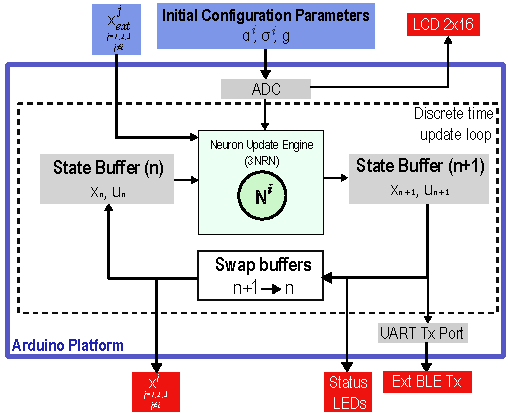
\includegraphics[width=\columnwidth]{Figures/fig_001_2.pdf}
\caption{Functional architecture of a single distributed embedded neuron node. Each node executes the local discrete-time nonlinear dynamics using a buffered state-update mechanism, while coupling signals from neighboring neurons are incorporated through external communication links. The resulting membrane-state signal is transmitted to adjacent nodes to preserve the coupled network dynamics during distributed real-time execution.}
\label{fig:001}
\end{figure}

\section{Hardware implementation on Arduino UNO} \label{Implementation}

To demonstrate that WLC can be exploited as a real-time information coding mechanism in embedded hardware, we implemented a three-neuron network based on the discrete-time non-chaotic Rulkov model (3NRN) using Arduino microcontrollers. The objective of this implementation is not to reproduce a biological system in detail, but to realize a low-cost neuromorphic platform in which distinct WLC regimes can be mapped into discrete motion commands.

The hardware architecture consists of three microcontroller-based neuron modules and a wireless communication stage. Together, the three neurons form a discrete nonlinear network that operates as a central pattern generator. For selected parameter configurations, the network produces sequential switching patterns associated with WLC-like dynamics, which are then associated with symbolic motion codes and transmitted to an actuator module through Bluetooth Low Energy (BLE) using an ESP32-WROOM TX--RX pair. The distributed hardware arrangement adopted for this proof-of-concept implementation is shown in Fig.~\ref{fig:003}.

\begin{figure}[t]
\centering
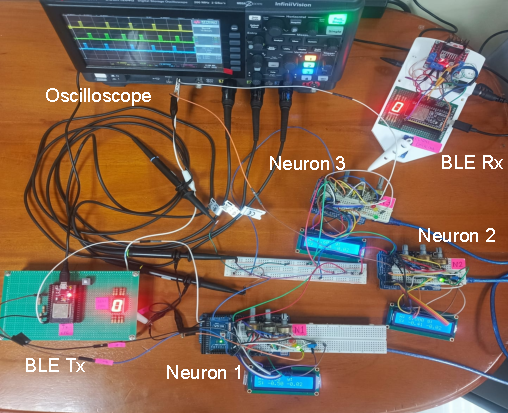
\includegraphics[width=\columnwidth]{Figures/fig_002.pdf}
\caption{Experimental distributed hardware prototype used for validation of the coupled nonlinear network. Each neuron is implemented on an independent Arduino-based embedded node with local parameter configuration, LCD monitoring, and inter-node coupling connections. The membrane-state signals exchanged between nodes are monitored using a digital oscilloscope, while an external BLE-enabled interface is used to transmit symbolic WLC codes to an external actuation module.}
\label{fig:003}
\end{figure}


Before hardware implementation, an offline parameter study was conducted to identify $(\alpha^i,\sigma^i,g)$ configurations that preserve WLC dynamics in the distributed network. In this study, the network configuration was restricted to a fixed phase shift in the parameter $\alpha^i$, such that $\alpha^3=\alpha^2+0.10=\alpha^1+0.20$, while $\sigma$ and $g$ remained identical across all nodes. From the experimentally validated WLC regions, four representative parameter configurations were selected and associated with symbolic codes $c\in\{0,1,2,3\}$. These codes were used as representative motion states during external interfacing experiments. The selected configurations were chosen to reduce ambiguity during manual parameter transitions and to minimize transient trajectories between neighboring dynamical regimes.

It is important to note that the embedded implementation does not perform real-time detection or classification of WLC dynamics. Instead, the system uses predefined symbol assignments associated with previously identified WLC parameter configurations. As an implementation guide, Table~\ref{tab:tuplas} summarizes the four experimentally selected parameter configurations associated with the symbolic motion modes used during distributed hardware validation. Each tuple corresponds to a previously identified WLC regime under the imposed phase-shift condition between neurons.

Although each neuron exhibits its own temporal evolution within the distributed WLC regime, once the sequential switching pattern is established, a single reference signal is sufficient to identify the corresponding symbolic state. In the present implementation, the membrane potential of neuron 1 is therefore used as the reference signal for symbolic code assignment and UART/BLE transmission. This choice simplifies experimental validation; future implementations will incorporate coordinated parameter updates or shared configuration interfaces across all neuron nodes.

The transmitter sends the assigned symbolic code through an external BLE component, while the receiver translates the incoming code into the corresponding actuator command.A 7-segment display is used to visualize the active code and verify TX--RX synchronization during operation. The control parameters $\alpha^i$, $\sigma$, and $g$ are provided through voltage dividers and digitized with 10-bit resolution. Internally, the platform supports floating-point values in the ranges $\alpha^1\in[4,10]$ with step size $0.10$, $\sigma\in[-0.5,0.5]$ with step size $0.01$, and $g\in[-0.1,0.1]$ with step size $0.01$. A display module shows the active parameter values, while three colored LEDs provide a direct visualization of the firing level of each membrane potential $x_{n+1}^i$ in real time. Analog input and output pins are used to emulate the synaptic couplings described by Eqs.~\ref{Eq5} and~\ref{Eq6}, enabling bidirectional interaction between neuron modules.

The complete system therefore integrates three functional layers: generation of WLC dynamics, temporal decoding into symbolic commands, and wireless transmission to an actuator stage. In this sense, the prototype serves as a minimal proof-of-concept, showing that sequential switching in a discrete nonlinear neuromorphic network can be used as an embedded coding strategy for real-time control tasks.

Figure~\ref{fig:impl003} compares, for each motion code, the simulated attractor, the corresponding membrane potential time series, and the oscilloscope recordings obtained from the Arduino implementation. The qualitative agreement observed between numerical and experimental signals supports the feasibility of reproducing WLC-like sequential dynamics on low-cost embedded hardware.

\begin{table}[htbp]
\begin{center}
\caption{Parameter tuples $(\sigma,\alpha^1,g)$ selected for each motion mode. For all modes, $\alpha^2=\alpha^1+0.10$ and $\alpha^3=\alpha^1+0.20$.}
\label{tab:tuplas}
\begin{tabular}{| c | c | c | c | c |}
\hline
Mode & Code & $\sigma$ & $\alpha^1$ & $g$\\
\hline
 Forward    & 0 & $-0.5$ & $6.5$ & $-0.02$\\
\hline
 Right Turn & 1 & $-0.4$ & $6.0$ & $-0.03$ \\ 
\hline
Left Turn  & 2 & $-0.2$ & $5.2$ & $-0.04$ \\
\hline 
 Standby    & 3 & $0.0$  & $4.0$ & $0.06$\\
\hline 
\end{tabular}
\end{center}
\end{table}

\begin{figure} [htbp]
    \centering
  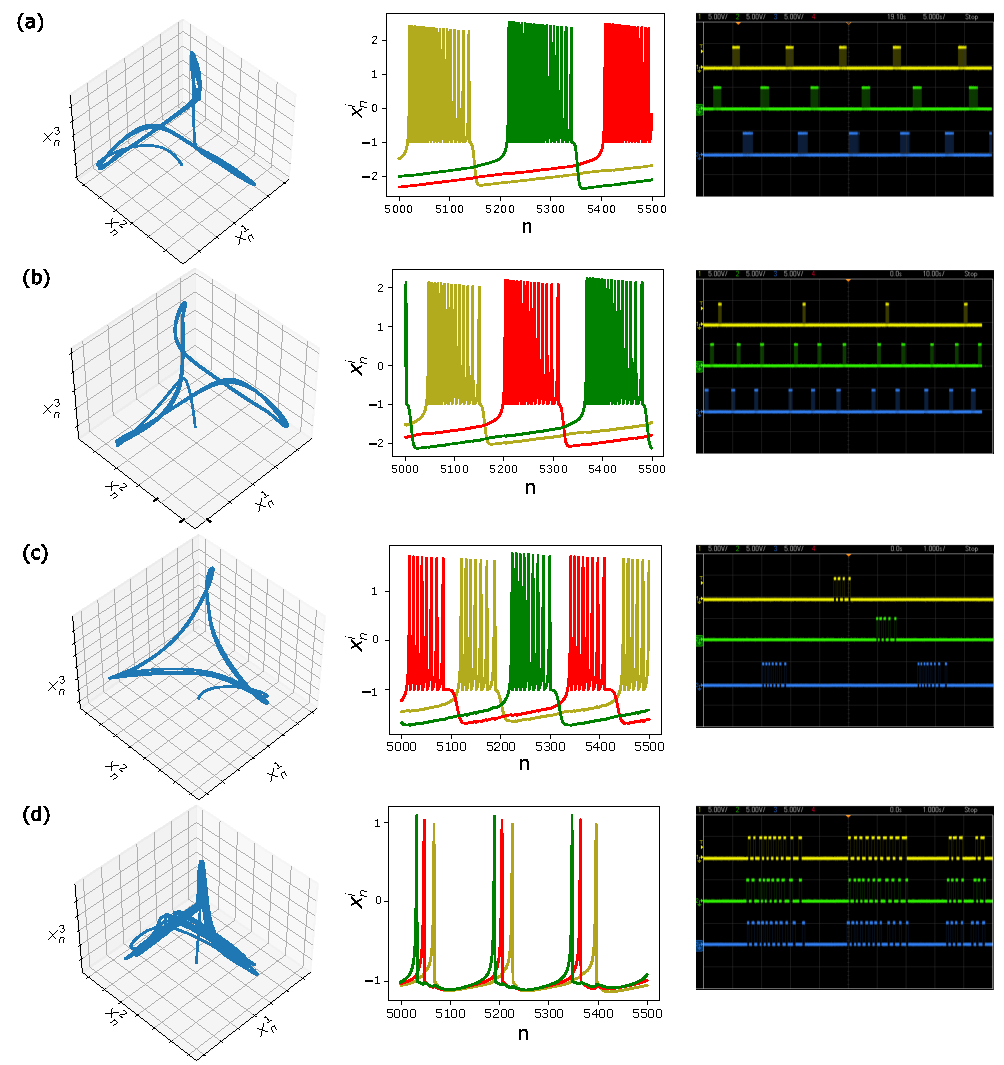
\includegraphics[width=\columnwidth]{Figures/Fig3.pdf} 
  \caption{\textbf{Simulated and experimental signatures of the embedded WLC-based coding scheme.} Each row corresponds to one motion code: (a) Forward (c=0), (b) Right Turn (c=1), (c) Left Turn (c=2), and (d) Standby (c=3). From left to right, the panels show the simulated attractor in $(x_n^1,x^2_n,x_n^3)$ space, the membrane-potential time series, and the oscilloscope recording obtained from the Arduino prototype. In the hardware implementation, each neuron is executed on an independent Arduino-based embedded node, where the coupled membrane dynamics are generated through distributed real-time state updates and inter-node signal exchange. The symbolic motion codes are not obtained through online dynamical classification, but through a predefined lookup-based mapping associated with experimentally selected WLC parameter configurations. 
  }
  \label{fig:impl003}
\end{figure}

\subsection{Robustness of the selected symbolic codes}

To evaluate the robustness of the selected symbolic codes, we performed a parameter sensitivity analysis around the experimentally selected operating points. Parameters $\alpha^1$, $\sigma$ and $g$ were independently perturbed using increments consistent with the effective resolution of hardware tuning, namely $0.1$, $0.01$, and $0.01$, respectively. The goal was to estimate the admissible variation range over which the WLC-like regime remains observable despite finite-resolution adjustment and small hardware-induced perturbations.

\begin{table} [htbp]
\begin{center}
\caption{Operating parameter intervals preserving the WLC regime around the selected symbolic codes.}
\label{tab:sensivity}
\begin{tabular}{| c | c | c | c |}
\hline
Parameter & $\alpha^1$ & $\sigma$ & $g$ \\
\hline
Code 0 &
$-$ & $[-0.49,-0.5]$ & $[-0.07,0.01]$  \\
\hline
Code 1 & $[5.7,6.0]$ & $[-0.44,-0.38]$ & $[-0.08,0.04]$ \\
\hline
Code 2 & $[4.7,5.3]$ & $[-1.19,-0.18]$ & $[-0.72,0.48]$ \\
\hline
Code 3 & $-$ & $[-0.22,0.08]$ & $[0.59,-0.40]$ \\
\hline
\end{tabular}
\end{center}
\end{table}

Table~\ref{tab:sensivity} summarizes the admissible variation margins obtained for the selected symbolic codes listed in Table~\ref{tab:tuplas}. The reported intervals indicate the parameter ranges within which a WLC-like regime is preserved around each operating point. The differences observed between codes suggest that robustness depends on the location of the selected operating point within the corresponding WLC region. For Codes 0 and 3, the selected values of $\alpha$ correspond to the boundary points of the WLC region. Consequently, no additional stable hardware adjustment steps were observed in the $\alpha$ direction within the potentiometer resolution explored ($\Delta\alpha=0.1$).
These results establish quantitative operating margins for validated symbolic states, providing an objective measure of robustness in the embedded implementation.

\section{Discussion}
Within this context, the proposed Arduino-based implementation provides, to our knowledge, the first hardware realization of WLC dynamics using a discrete non-chaotic Rulkov network on an accessible embedded platform. Beyond reproducing sequential switching patterns associated to the WLC regime, this implementation enables the identification and proof-of-concept of parameter configuration capable of generating distinct symbolic codes.

Unlike FPGA-based realizations \cite{caluwaerts2013tensegripede}, which generally require hardware description languages and dedicated design environments, the proposed implementation is based on the open-source Arduino platform and standard C/C++ programming. This reduces the complexity of development and facilitates reproducibility, making the experimental study of WLC dynamics accessible to a broader research community. The architecture operates through multiple independent Arduino nodes and therefore inherently includes communication delays, hardware-induced disturbances, and variation in the analog input configurations as part of real experimental conditions. Despite its simplicity architecture and non-ideal effects, the platform successfully reproduces the key dynamical features predicted by the numerical model under real operating conditions.
The hardware sensitivity analysis was consistent with the numerical WLC region maps, showing that the stability margins depend on the location of the selected operating point within the corresponding WLC region. This result indicates that the embedded implementation preserves the qualitative structure of the underlying parameter space.

\section{Conclusion}

This work presented a distributed embedded implementation of a three-neuron nonlinear network based on the discrete-time non-chaotic Rulkov map using multiple Arduino UNO nodes. In contrast to centralized implementations, each neuron was executed on an independent embedded platform, and both local state evolution and inter-neuron coupling were achieved through real-time signal exchange between physical devices.

The proposed architecture incorporated buffered state synchronization to preserve consistent temporal evolution under distributed execution constraints. Experimental results showed that the embedded network reproduced the sequential switching behavior associated with the WLC regime previously identified in numerical simulations, despite the presence of finite-precision arithmetic, communication delays, and hardware-induced perturbations.

The achieved WLC dynamics across independently tuned hardware nodes suggest a certain tolerance to the small parameter mismatches presented normally by embedded implementation. In addition, a hardware-oriented sensitivity analysis provided quantitative stability margins for the experimentally selected symbolic configurations, showing that the desired WLC dynamics can be maintained under small parameter variations consistent with the resolution of the embedded implementation. In this sense, the present system provides a proof of concept for the physical realization of WLC-like dynamics in a low-cost distributed embedded platform. 

The symbolic encoding layer associated with the experimentally selected WLC configurations enabled straightforward interfacing with external systems through lightweight communication modules. This feature illustrates the potential of discrete-time nonlinear dynamics for simple embedded control and signaling tasks.

Future work will focus on the development of systematic parameter-selection strategies to identify codes in WLC regions to maximize robustness under hardware restrictions, prioritizing operating points located deeper within the WLC region. Additional research will address automated parameter synchronization between nodes, larger network topologies, and sensor-driven adaptive implementations to further explore the use of WLC-based dynamics in embedded control and computation systems.
\ifCLASSOPTIONcaptionsoff
  \newpage
\fi
\bibliographystyle{IEEEtran}
\bibliography{IEEEabrv,Bibliography}
\begin{IEEEbiography}[{
\includegraphics[width=1.1in,height=1in,clip,keepaspectratio]{Photo/LPO_foto1.jpg}}]{Luis Pab\'on-Orozco} received the Electronic and Telecommunication Engineering degree from the Escuela Superior Polit\'ecnica del Litoral (ESPOL), Guayaquil, Ecuador, in 2013, and the Master degree in physics from Universidad Central de Venezuela (UCV) in 2025. He is a Professor at Dept. of Physics, Escuela Superior Politécnica del Litoral, Ecuador. His research interests include nonlinear dynamical systems, neuromorphic-like prototypes, and physics education using low-cost 3D printed prototypes.
\end{IEEEbiography}
\vfill
\begin{IEEEbiography}[{
\includegraphics[width=1.1in,height=1.in,clip,keepaspectratio]{./Photo/EDGM.jpg}}]{Esther D. Gutiérrez M} received a bachelor’s degree in physics with a concentration in computational physics at University Central of Venezuela (UCV) and a PhD in physics from the Venezuelan Institute for Scientific Research (IVIC) in 2015. She is a professor at the Dept. of Physics at
Escuela Superior Politécnica del Litoral, Ecuador. Her research interests focus on nonlinear dynamics, complex systems, stochastic dynamics, time series analysis, neural networks, machine learning, and physics education.
\end{IEEEbiography}
\vfill
\end{document}
